% SIAM Shared Information Template
% This is information that is shared between the main document and any
% supplement. If no supplement is required, then this information can
% be included directly in the main document.

As pointed out in the previous section parallelization of \SymmSpmv and \SYMMKACZ kernels can be done on basis of \DTWO coloring of the corresponding graph and the computational intensity, \ie the performance depends on the data access patterns of the kernels. As coloring schemes change data access patterns, they may interact with the computational intensity and we thus investigate this effect in more detail now. We apply  the basic multi-coloring scheme generated by COLPACK~\cite{COLPACK} to parallelize \SymmSpmv and compare it with \SpMV which serves as our performance yardstick. In~\cref{fig:motivation} we present performance measurements and data transfer volumes for the Spin-26 matrix on a single socket of the \IVB system. For basic \SpMV we recover the well know-memory bandwidth saturation effect as we fill the chip (~\cref{fig:motivation} (a)). Measuring the actual data volume from main memory using \LIKWID we find a value of $16.26$ Byte per non-zero matrix entry (~\cref{fig:motivation} (b)). This value corresponds to the denominator of $I_\mathrm{\SpMV}$ in~\cref{eq:SpMV_intensity} and we can calculate $\alpha_\mathrm{\SpMV}=0.353$. Along the discussion in~\cref{sect:SymmSpmv} using the load-only bandwidth of \IVB (see~\cref{tab:test_bed}) we find a maximum attainable {\SymmSpmv} performance for this matrix of $P^{max}_\mathrm{\SymmSpmv}=8.95$ \GF; see~\cref{eq:SymmSpMV_performance}. While this value indicates a speed-up of approximately 1.6$\times$ compared to \SpMV yardstick (approx. $5.5$ \GF on the full socket), the \SymmSpmv implementation using \MCfull (\MC) only achieves a fraction of that and is more than three times slower than \SpMV. 



  \begin{figure}[thbp]
  	\centering
 % 	\subfloat[SpMV]{\label{fig:motivation_spmv}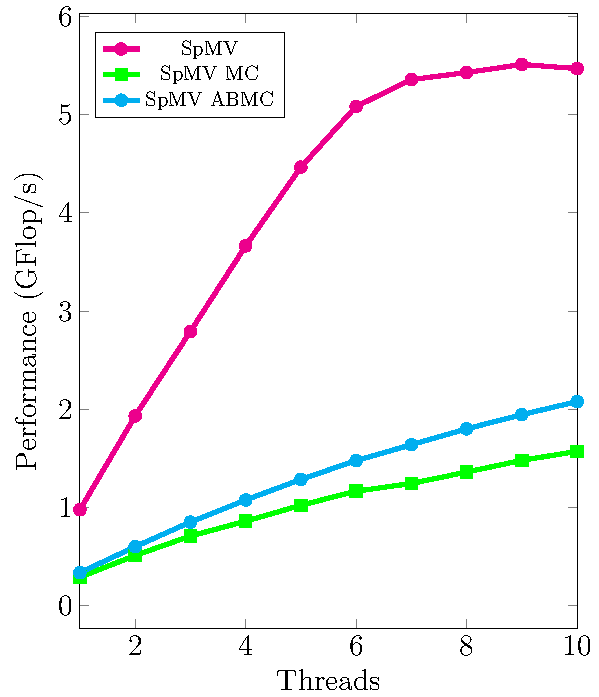
\includegraphics[width=0.26\textwidth, height=0.22\textheight]{pics/motivation/out/motivation_spmv}}
  %	\hspace{1em}
    \subfloat[SymmSpMV]{\label{fig:motivation_symm_spmv}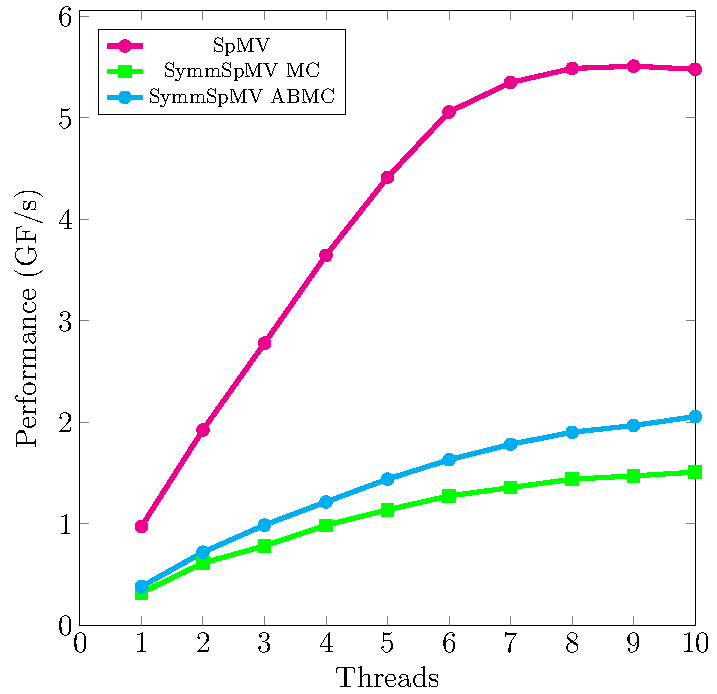
\includegraphics[width=0.38\textwidth, height=0.22\textheight]{pics/motivation/out/motivation_symm_spmv}}
    \hspace{1em}
  	\subfloat[Data Traffic]{\label{fig:motivation_data}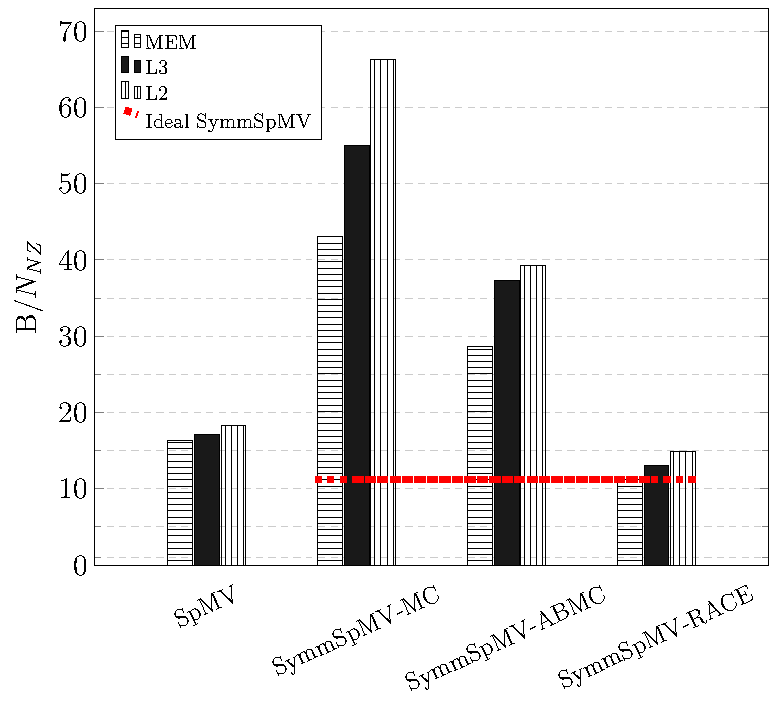
\includegraphics[width=0.4\textwidth, height=0.22\textheight]{pics/motivation/out/motivation_data_w_RACE}}
  	
  %	\subfloat[False sharing]{\label{fig:motivation_c}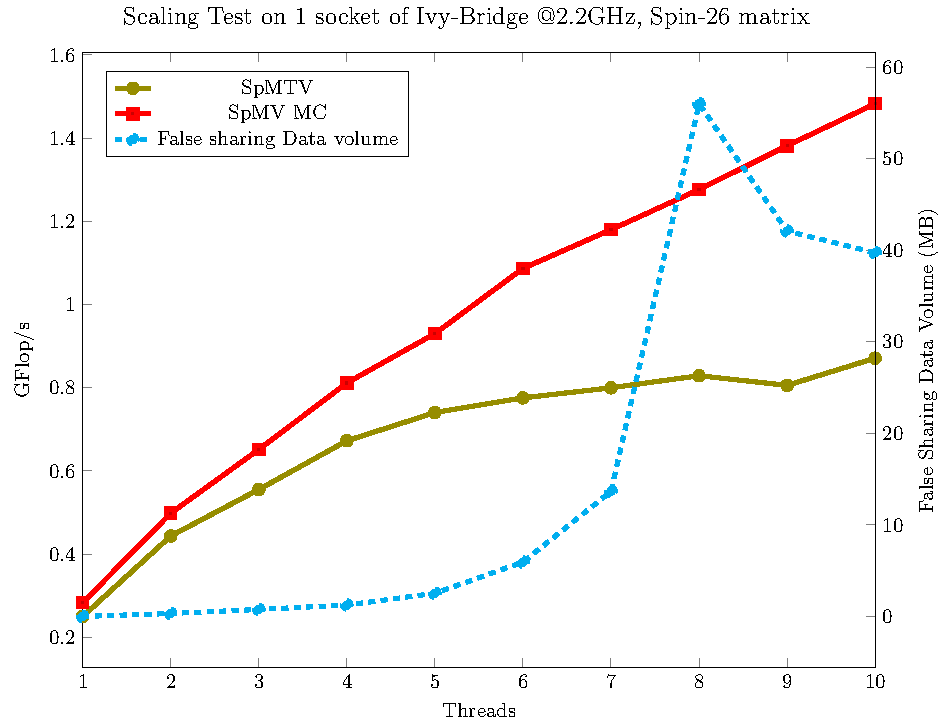
\includegraphics[width=0.45\textwidth, height=0.22\textheight]{pics/motivation/motivation_2}}
  %	\hspace{1em}
  %	\subfloat[Barrier effect]{\label{fig:motivation_d}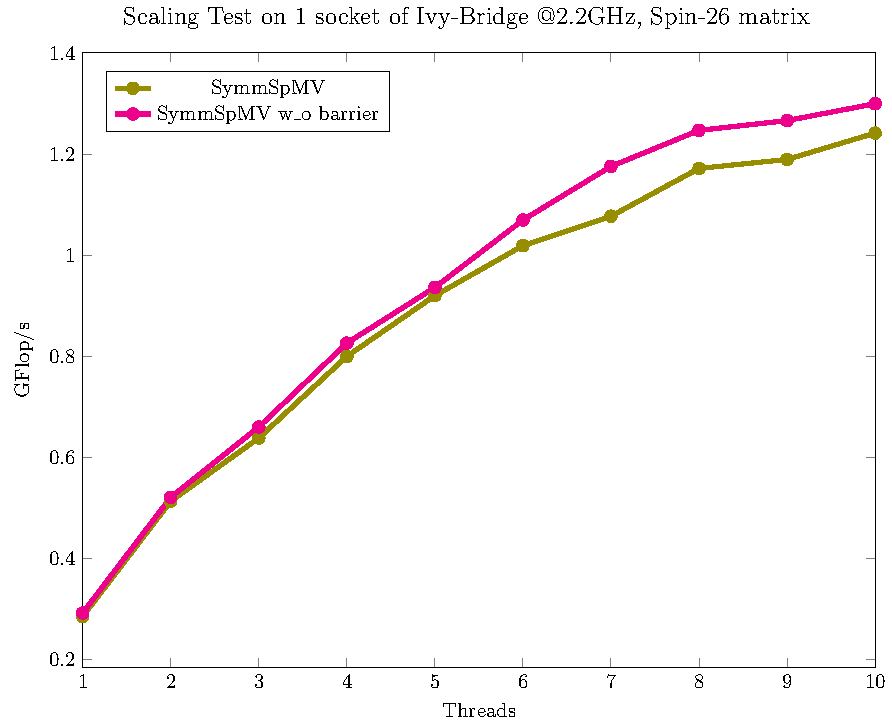
\includegraphics[width=0.45\textwidth, height=0.22\textheight]{pics/motivation/motivation_4}}
  	\caption{\Cref{fig:motivation_symm_spmv} performance of \SymmSpmv with \MC and \ABMC compared to \SpMV performance, \cref{fig:motivation_data} average data traffic per non-zero entry ($\NNZRmath$) of the full matrix as measured with \LIKWID for all cache levels and main memory. Note that all the measurements were done on \IVB socket at 2.2GHz. For all the methods matrix was pre-permuted with \RCM }
  	\label{fig:motivation}
  \end{figure}
 
\begin{comment}
{\GW Original Text - bitte auskommentieren
Motivation for developing an alternative method stems from the ESSEX (Equipping Sparse Solvers for Exascale) project \cite{ESSEX}
 where we investigate into solving large eigen-value problems from quantum mechanics field. In this context having a robust iterative solver was inevitable, due to the poor condition number of the matrices that appear in this field. Kaczmarz (\KACZ) solver was found to be satisfactory but parallelizing this solver was deemed challenging because of the loop-carried dependencies in the kernel. Previous work on parallelizing the \KACZ kernel used \MCfull (\MC) \cite{feast_mc} but it was soon found that the kernels do not scale efficiently with this approach.
In order to get a better understanding of the underlying problem it's convenient to choose simple symmetric sparse matrix vector (\SymmSpmv) as a benchmark kernel. The particular choice of this kernel is due to the fact that both \KACZ and \SymmSpmv have similar kind of dependencies, and it's much easier to compare with our reference kernel namely sparse matrix vector (\SpMV) which is embarrassingly parallel. The algorithm for \SymmSpmv  and \SpMV has been listed in \cref{alg:SymmSpMV,alg:SpMV}}
 \Cref{fig:motivation_spmv} shows the performance of \SpMV kernel on original unpermuted matrix and matrix with \MC permutation. Here we see the performance of \SpMV on multicolored matrix is  four times  worse than that of  \SpMV on unpermuted matrix. One of the major reason for this drop is due to the increase in $\alpha$ factor seen in the intensity equation \cref{eq:SpMV_intensity}  Since the kernels like \SpMV  are mainly memory bound increase in $\alpha$ lowers intensity $I_\mathrm{\SpMV}$ leading to a drop of performance as predicted by \roofline model \cite{Williams_roofline}. This could easily be demonstrated by measuring the data traffic between different memory hierarchies.  We do this using the \LIKWID tool \cite{LIKWID}, and the measurements can be seen in \cref{fig:motivation_data}. One can see an increase in data-traffic from all the memory hierarchy compared to \SpMV on normal unpermuted matrix. This is basically caused by the bad data locality introduced by \MCfull permutation.
\end{comment}
%  \begin{figure}[htbp]
 % 	\centering
  %	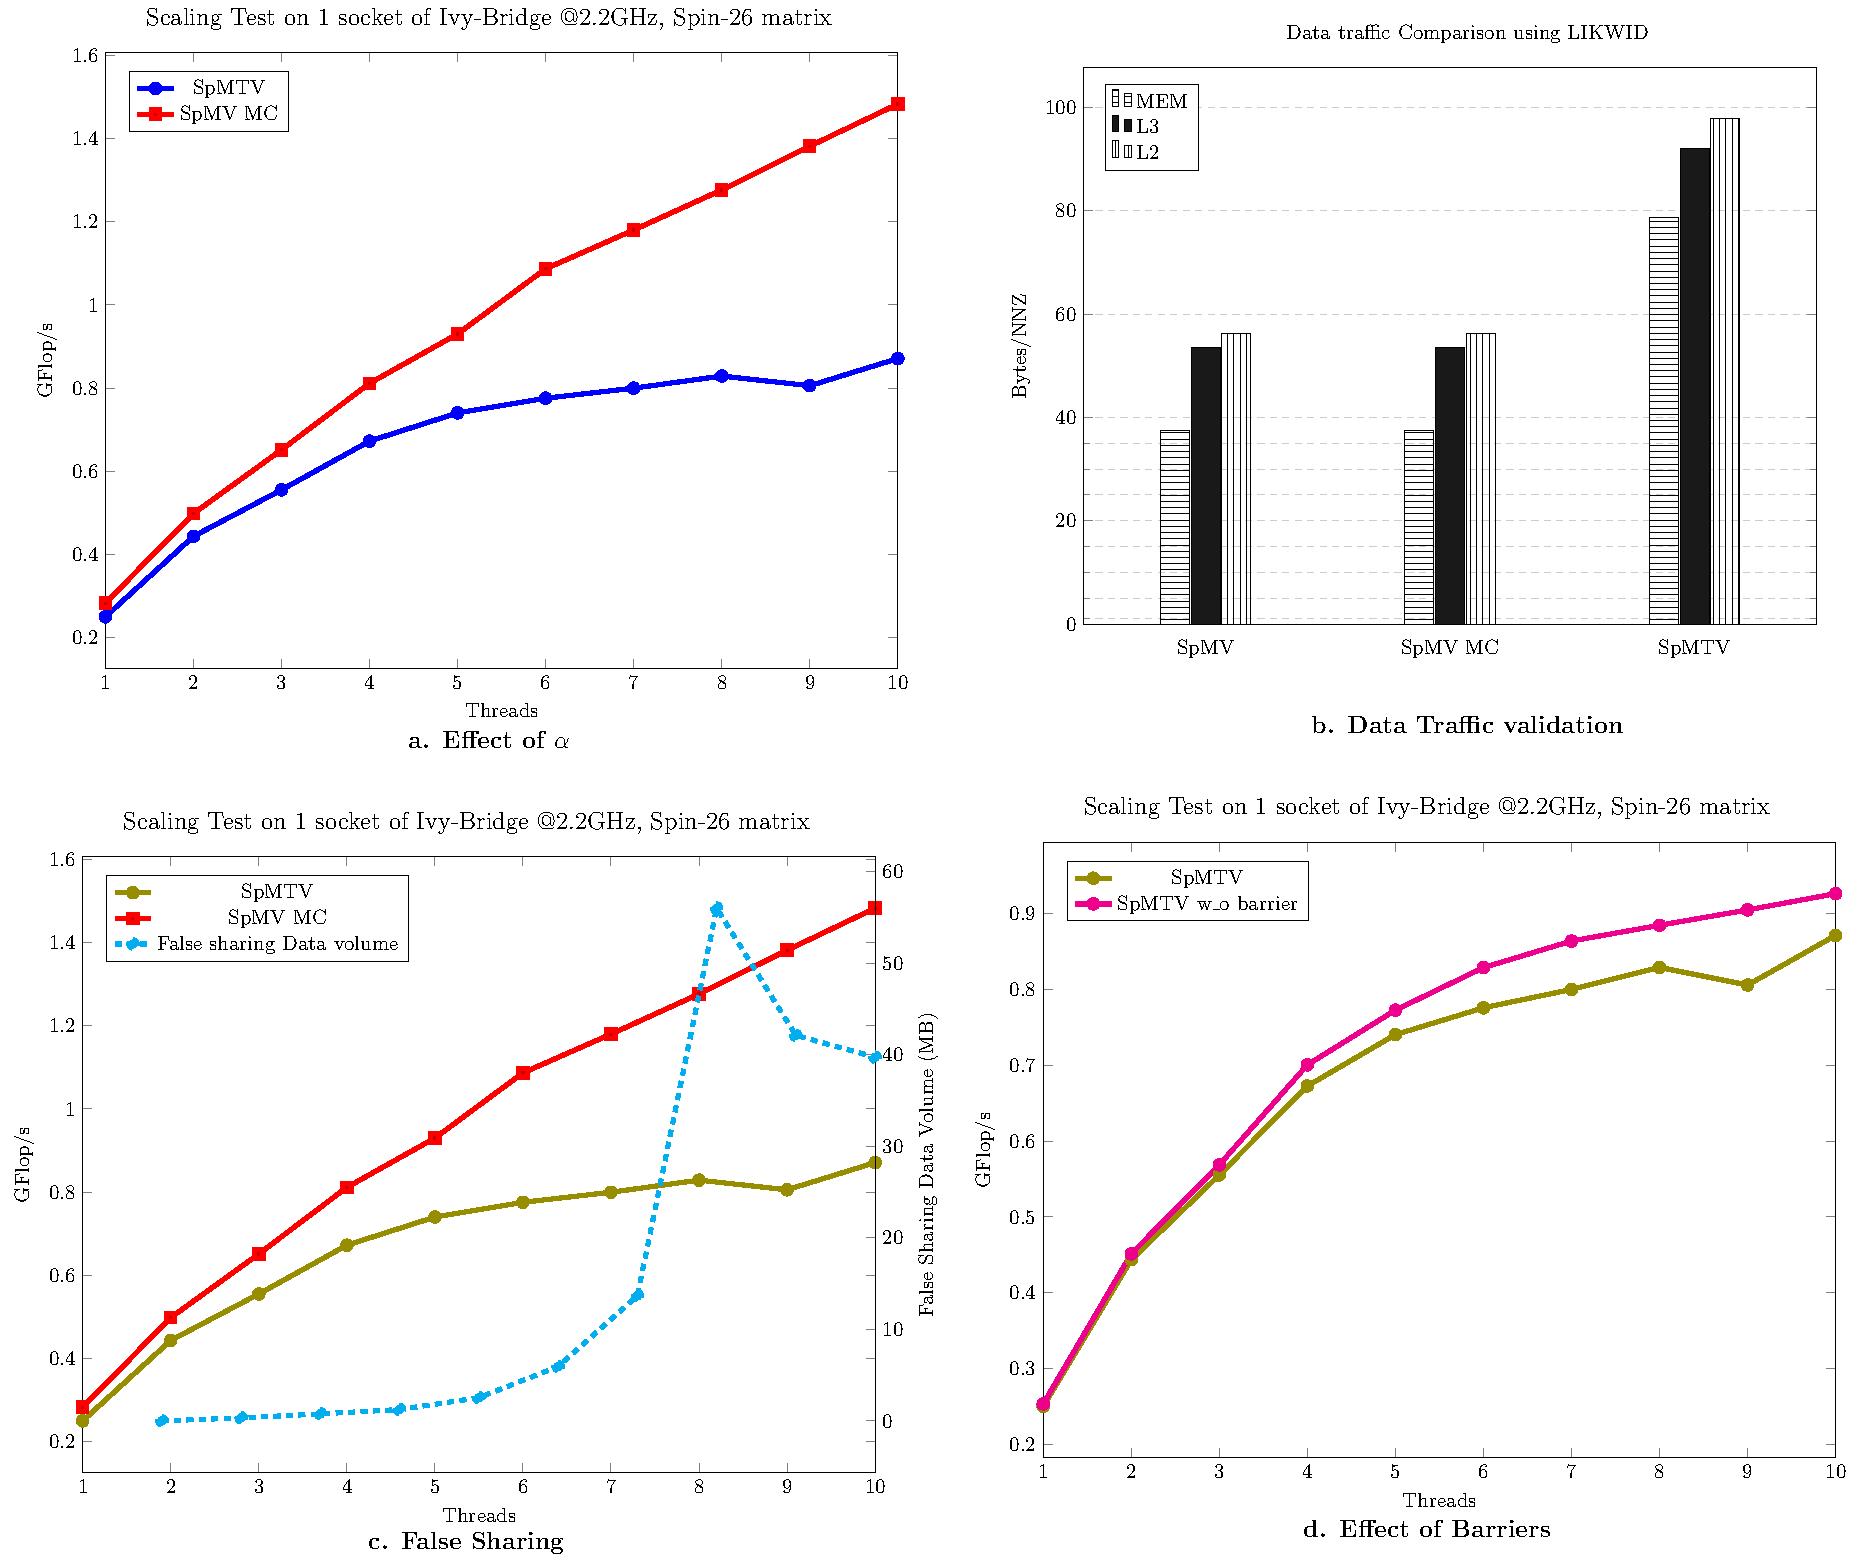
\includegraphics[width=0.9\textwidth, height=0.4\textheight]{pics/motivation/motivation}
  %	\caption{Illustration of increase in $\alpha$ by multicoloring, numbers represents thread numbers working on a particular row}
  %	\label{fig:motivation}
  %\end{figure}
  \begin{figure}[htbp]
  	\centering
  	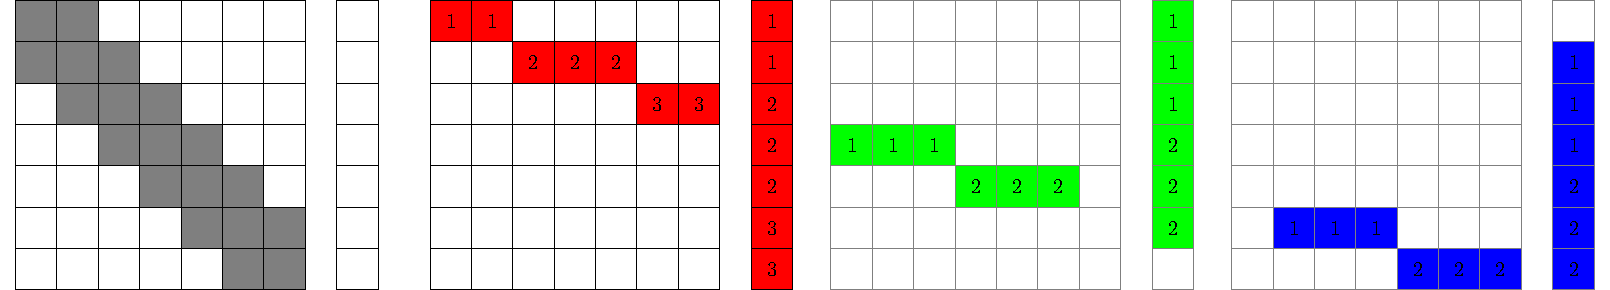
\includegraphics[scale=0.45]{pics/mc_alpha_problem/mc_alpha_unsymm}
  	\caption{Illustration of increase in $\alpha$ by multicoloring, numbers represents thread numbers working on a particular row. Please note that \cref{fig:mc_alpha} shows only rows of the matrix permuted according to \MCfull but in actual practice one would do this permutation symmetrically \ie both rows and columns are permuted.}
  	\label{fig:mc_alpha}
  \end{figure}
  
  The basic reason for this is the nature of \MCfull (\MC) permutation. For \DTWO \MC sets of structurally orthogonal rows have to be determined \cite{dist_k_def}, \ie rows that do not overlap in any column entry. Then different colors are assigned to each set. \Cref{fig:mc_alpha} shows corresponding permutation applied to a toy problem with high data locality and the obtained sets of colors. Rows within a color can be executed in parallel but colors are operated one after the other. However now a color may contain rows from very different parts of the matrix potentially destroying data locality of the original matrix.  Assuming last level cache (\LLC) can hold a maximum of six elements we find for every new color we need to load right hand side vector every time for each new color. This is the reason why we observe 3$\times$ more bytes per \nnz for \SymmSpmv with \MC compared to \SpMV as seen in~\cref{fig:motivation_data}.  However our performance model indicates that \SymmSpmv should achieve a traffic of only 0.7$\times$ that of \SpMV (see red dotted line in \cref{fig:motivation_data}). Of course it is obvious this effect strongly depends on matrix structure, matrix size and cache size. 
      
  
  Algebraic Block \MCfull (\ABMC) tries to preserve data locality by first partitioning the entire matrix to blocks of specified size and then applying \MCfull to these blocks. Along the lines of \cite{Park_HPCG} we use \METIS \cite{METIS} to partition the matrix into blocks. Threads then work in parallel between blocks of the same color. This reduces data traffic (see \cref{fig:motivation_data}) as there is better data locality within a block. Consequently the performance improves over \MC method (see \cref{fig:motivation_symm_spmv}). But still we are far off the performance model prediction of 8.95~\GF.
  
  In addition to data locality other factors like global synchronizations and false sharing also contribute to the performance drops. These factors strongly depend on the number of colors and in general increase with chromatic number. For the Spin matrix the overhead of synchronization is roughly 10\% for \MC method.  For most of the matrices considered in this work one could also observe a strong positive correlation between false sharing and number of threads for \SymmSpmv kernels, due to the indirect writes in \SymmSpmv.
 
 %As seen in \cref{fig:motivation_data} the data traffic further increases for \SymmSpmv, although ideally one would expect only half the data traffic as \SpMV since we operate only with upper triangle part of the matrix. The reason for this extra traffic is due to additional indirect writes (scatter) and this scales up $\alpha$ factor as seen in the denominator of $I_{\SymmSpmv}$ (see \cref{eq:SymmSpMV_intensity}),  which further decreases performance of \SymmSpmv compared to \SpMV on \MC matrix. Note that ideal performance of \SymmSpmv is almost twice as that of \SpMV if the code could saturate the memory bandwidth.
 


%Overall for all the matrix in our test-suite it was seen that average drop in performance by \MCfull was almost a factor of two on a single socket of \IVB. Although for most of them performance could be improved by \ABMCfull (\ABMC), still the results we obtained were not optimal (especially for large matrices) when compared to performance models which we will see later in \cref{Sec:expt}. This led to the development of a method which works on a common data format like \CRS in which most of the other kernels are written and at the same time preserves data locality, reduce synchronization overheads and false sharing. 

In the following we address the above mentioned problems and formulate an improved hardware friendly coloring method called \RACfull (\RAC) to alleviate these issues. This leads to substantial performance improvements, as seen in the case of Spin-26 matrix. Here we achieve close to optimal data traffic and a performance of 7.3 \GF(see \cref{fig:motivation}) which corresponds to 82 \% of our performance model using load-only bandwidth.

 

